\section{Real World application}

A general s-plex application that is probably used is the identification of group or friend networks
where one can make assumptions about group or friend networks. This is application is not directly
derived from our programming assignment, but it is somewhat related since one still has to identify k-plexes in a
undirected graph which with the amount of people using social media these days is not trivial.
An application that is closer to the given s-plex programming assignment would be telecommunication networks.
Where the distance between the antennas, towers or compute node could be correlated to the weight matrix and the s-plex
relaxation of the clique's could be used to make crucial system more reduntant (low s-plexes) and other less crucial systems
less reduntant (higher s-plexes).
\section{Introduction}
\subsection{Notation}
For brevity we use the following notation here in the report and in the code.
\begin{enumerate}
    \item We call our solutions $G$ and the number of nodes $n$.
    \item We call the original Adjecency Matrix of the given graph $A_0$ and the one of our solution $A$. We call the weight matrix $W$.
    \item we call a connected subgraph (so a set of nodes that are all directly or indirectly connected by edges and that have no edges going out of the set) a \textbf{cluster}.
\end{enumerate}

\subsection{State of the project}
The code and the experiments are in a very "raw" state as we submit them. The code could still be greatly cleaned up and optimized. Our function names, signatures and return values are not uniform, which might be confusing sometimes. Here is our justification:\\
First we want to say that we really enjoyed this project and that we had a lot of fun working on it. We put a lot of time in the project at this point and we are happy with our results. We would like to spend 2 more weeks on it to learn more about the problem and to see how far we can take this. However, this project only makes up 20\% of a 4.5 ects course and we have many other obligations so we can not spend as much time on it as we want. We therefore hope that the raw form of the submission is okay.\\

\subsection{MHLib}
We originally planned to use MHLib in our project. We did get the library running on our instances, which you can test in \texttt{gvns\_mhlib.jl}. At some point we decided that it would be easier to implement the metaheuristics ourselves so in the following we are using our self-implemented metaheuristics. At some points in the code you will find artifacts of us trying to use MHLib, like the function \texttt{calc\_objective} and so on. Still we are happy that we tried to use MHLib because this made us get to know julia and we really like the language!\\

\subsection{Hardware and Setup}
We ran all experiments on our local machines with the following specifications:
\begin{itemize}
    \item intel i9-12900H on WSL2 on Windows 10 with julia 1.9.3
    \item intel i5-10310U on WSL2 on Windows 11 with julia 1.9.3
\end{itemize}
We will specify which data is taken on what machine in the experiments section.

\subsection{Experiments}

Due to time constraints we did not let all algorithms run on all instances. We have results for the VND algorithm for all instances but not for GRASP and GVNS. Running all instances with reasonable numbers of iterations (both for GRASP and GVNS) would have taken mutliple days. We therefore only ran GRASP, GVNS and local search on the competition instances and the rather "fast" instances.\\
Also due to time constraints, we did not use best practice for experimentation. We did not let our experiments run mutliple times to take averages and standard deviations of the running time. We know that this could be done much better but again, we think for a 20\% of 4.5 ects project it is okay.

\section{Real World application}

A general s-plex application that is probably used is the identification of group or friend networks
where one can make assumptions about group or friend networks. This is application is not directly
derived from our programming assignment, but it is somewhat related since one still has to identify k-plexes in a
undirected graph which with the amount of people using social media these days is not trivial.
An application that is closer to the given s-plex programming assignment would be telecommunication networks.
Where the distance between the antennas, towers or compute node could be correlated to the weight matrix and the s-plex
relaxation of the clique's could be used to make crucial system more reduntant (low s-plexes) and other less crucial systems
less reduntant (higher s-plexes).

\section{Basic Ideas behind the algorithms}
\label{sec:basic_ideas}

\subsection{Construction heuristic}
\label{const_idea}

Our first idea for a construction of solutions is the following: An empty graph (without edges) is always a 1-plex, since a single node without edges is a 1-plex. Removing all the edges gives a valid solution, however a very bad one. Our first idea for an algorithm that finds a good solution was to start with an empty graph and go through all the edges in $A_0$, check if adding them to $A$ is legal and if so, do that. This algorithm improves the empty graph, however it can only find $s$-plexes of up to $|S|=s+1$. The reason is that it will connect the first node $v_1$ with $\min(s,\deg_{A_0} (v_1))$ many other nodes, then the cluster of $v_1$ is an $s$-plex with size at most $s+1$ and no more nodes can be added. Then, all the other nodes in the cluster might get connected among each other, but the $s$-plex will not get any bigger. Practically speaking, with this construction we got approximately $n/(s+1)$ many clusters of size $s+1$ which were mostly fully connected, so this construction results in small clusters.\\
For our radom construction we randomly parse the entries of $A_0$ but do the same as above otherwise.\\

Here we want to give a brief history of how we came up with the presented algorithms and why we think they are a reasonably good solution to the given problem.\\

\subsection{Local improvement move operators}
After this point we found it difficult to think of the next move, because simply adding one edge in this state will always yield an illegal solution. In trying to understand the problem better, we wrote the adjacency matrices $A_0$ in files and looked at their structure. What we found was that there is a structure in most of the graphs, more precisely there are 3 types of graphs (see also figure \ref{fig:types}):
\begin{enumerate}
    \item locally strongly connected: 26/60 (Here, nodes that are close in numbering are also strongly connected in the graph)
    \item seemingly randomly connected: 23/60
    \item tentacle-like connected: 7/60 (Here, the Graphs have a semi-large, strongly connected cluster with "tentacles" reaching out. Tentacle-shaped clusters are bad for $s$-plexes, so we will have to seperate these "lines" into small "spheres".)
\end{enumerate}

\begin{figure}[h]
    \centering
    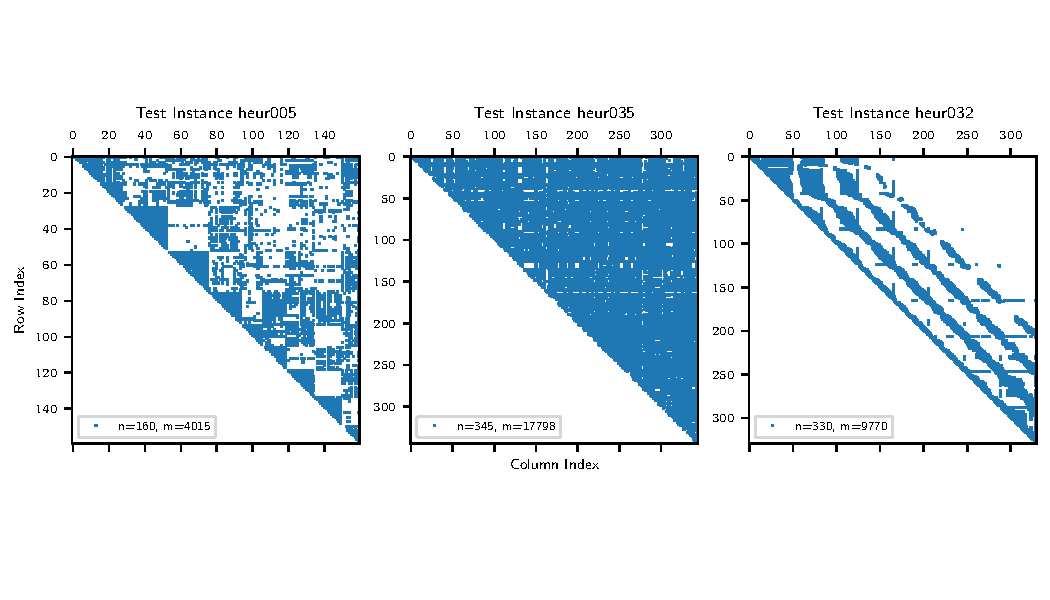
\includegraphics[width=\linewidth, trim= {0 1.8cm 0 1.8cm}, clip]{figures/spy_adjacency.pdf}
    \caption{\label{fig:types}Instances of the different graph types. Left is a locally strongly 
    connected graph, this is part of instance 005. In the middle is a seemingly randomly connected graph, 
    which is part of instance 035. On the right is a tentacle-like connected graph, which is part of instance 032.}
\end{figure}

We will use this special structure of some instances to derive parts of our algorithms. Some might consider this cheating, but we think, that finding patterns in the instances is an important part of solving problems in real world applications so we find it to be okay. We will see later, that for the locally strongly connected instances we can find reasonably good solutions with very little computational effort. We will also see that the algorithms that were derived with the locally connected graphs in mind also work well on the other graphs.\\

\subsubsection{Fuse Operation}
The case of locally strongly connected graphs made it easier to think about the problem. The idea for our next move came from looking at the following situation. Let's say we are looking for 2-plexes and a certain section of our adjacency matrix is a clique, so $A_0$ in that part looks like\\
0111110\\
0011110\\
0001110\\
0000110\\
0000010\\
0000000\\
Our construction will find\\
0110000\\
0010000\\
0000000\\
0000110\\
0000010\\
0000000\\
To get from our constructed $A$ to $A_0$ in this section we need to set to 1 all the entries between the 2 cliques. In terms of the graph, we fully connect the two found cliques. Exactly this is our idea for the first move, which is then also applicable for the randomly distributed graphs.\\
So our first move after construction is fully connecting existing clusters, this always yields a legal $s$-plex. We call this operation a \textbf{fuse} the corrsponding functions are called \texttt{fuse\_first!} for first improvement and \texttt{fuse\_best!} for best improvement. We implemented this operation in a way, that it can fuse any 2 clusters, not only neighbouring ones.\\
Especially for the locally connected instances we found this to work very well and after repeatedly fusing clusters, our found adjecency matrices $A$ showed very similar structures to the original ones $A_0$.\\
After fusing two clusters one could also try to remove edges that are not there in $A_0$ until no more edges can be removed legally. We describe our strategy for this in section \ref{sec:cliquify}. To do this after every move, set the global variable \texttt{SPARSEN} to true in \texttt{move\_ops.jl} (as we said above: the code is very raw). We found that setting this to true improves the results slightly but greatly decreases performance (but we should mention here that we also implemented this in a very inefficient way). We decided that for good results it is sufficient to let the fuse method fully connect it's clusters and only at the end of the algorithm take out the unnecessary edges (see section \ref{sec:cliquify}).

\subsubsection{Swap operation}
Looking at our results we found that in some cases, single nodes did not land in the cluster they were supposed to be in, for example in the case of instance 051 we found the solution given in figure \ref{fig:051_swap}\\

\begin{figure}[h]
    \centering
    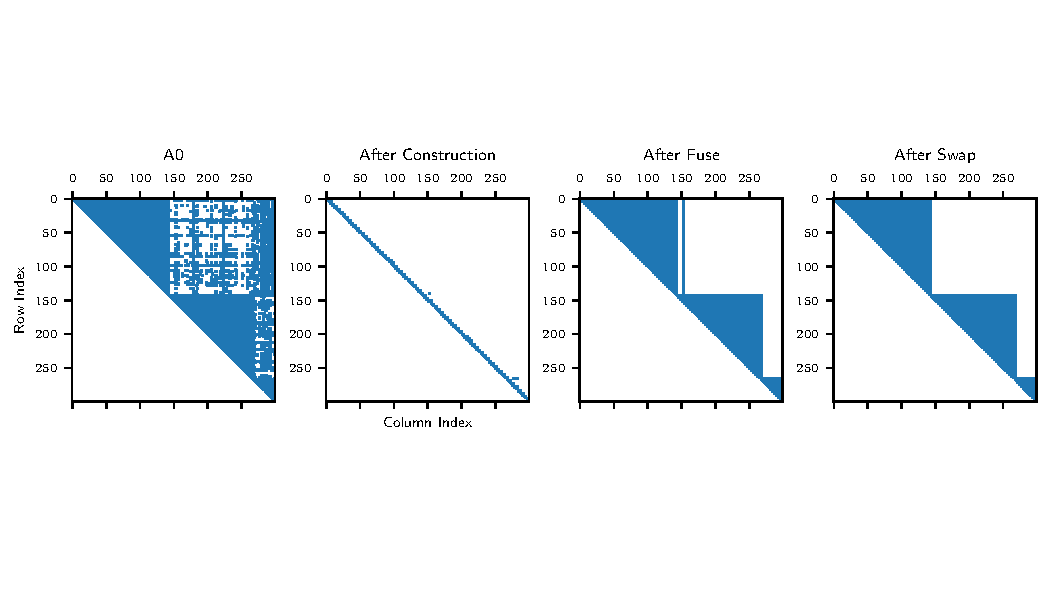
\includegraphics[width=\linewidth, trim= {0 1.8cm 0 1.8cm}, clip]{figures/spy_adjacency2.pdf}
    \caption{\label{fig:types} Instance 051 after fusing until no progress is made. One can see that node 
    154 seems misplaced. Indeed, when node 154 is swaped to the other cluster the cost is reduced by roughly 500.}
\end{figure}

We see that node 154 looks a little misplaced and should be in the first cluster note the second one. When we manually put it into the first one we found that this indeed reduced the cost from 8584 to 8087 which is a very significant improvement. So for our second move we think that it should be beneficial to try to swap nodes between clusters.\\

\subsubsection{Operation for taking out redundant edges}
\label{sec:cliquify}
All the discribed algorithms so far rather find cliques than s-plexes. In the fuse method, the clusters get fully connected, so any deviation from a clique must be in the original small clusters from the construction heuristic. Our algorithm finds clusters that are also clustered in $A_0$ but up till now it does not deal well with the edges in $A_0$ that are missing within a cluster. Generally, the most profitable edges in a cluster to remove will not always be in the small cluster from the construction heuristic. To find these most profitable edges to remove we implemented the \textbf{cliquify then sparsen} method. This method first fully connects the clusters within $A$ and then removes as many edges as possible, starting from the most profitable edges. This does not really fit into the framwork of metaheuristics, that we saw in the lecture, since it is more of a "cleanup" at the end of the search algorithm. One could also do one \textbf{cliquify then sparsen} after each however, this is again connected to more computational effort.\\
\subsubsection{Final thoughts}
In the case of the locally strongly connected graphs, our deterministic construction with a first improvement fuse strategy already works very well while being very efficient. The deterministic construction which goes through the nodes by their numbering and thereby clusters them mostly right, since nodes that are close in numbering are also "close" in the graph. The first improvement fuse operation will then first fuse the clusters which are closest in numbering, which also fits the structure of these graphs.\\
In the case of seemingly randomly connected graphs, the numbering is not correlated to how close nodes are in the graph, so here a random construction with GRASP, that rather randomly groups nodes in the beginning should perform better. For the same reason, a best improvement strategy for the fuse-operation should be better, however, this is very costly in terms of computation.\\
From our discussion above, we come to the conclusion, that first progressively fusing clusters until there is node more profit to make from fusing and then swapping the misplaced nodes until there is no more profit to make is a reasonable strategy here. Since there was no metaheuristic discussed in the lecture that exactly fits this procedure we will call it \textbf{sequential local search} (SNS) because we sequentially apply move operators. It is very close to VND, except it can not do fuse operations any more once it is finished with the fuse neighbourhood. We will compare this metaheuristic to the other ones. Our expectation is that the results will be slightly worse than for e.g. VND but that the computational performance will also be slightly better.\\
\subsubsection{Shaking operation}
For the shaking operation for GVNS we thought that randomly disconnecting $n$ nodes totally might be a good idea. We implemented this an we will discuss it in the results section.\\

\section{Construction Heuristic}

We used the idea of section \ref{const_idea} to implement our construction heuristic. You can find the implementation in the functions \texttt{det\_const!} and \texttt{rd\_const!}. One result of our construction heuristic is shown in figure \ref{fig:051_swap}. You can see that the algorithm only finds very small clusters of nodes, so we don't find the results of our heuristic worthy of experiments or a discussion. The objective values are, of course, poor but the runtime is very small.\\

\section{Local search}

For local search, both the fuse and the swap operator are feasible to use. Using the fuse operation is very fast (in terms of computation time) but gives rather poor results. The swap operator gives good results but it's computational performance is very poor. To conclude, as standalone moves for local search both are very poor. Both moves can be used in a first improvement and in a best improvement version.\\
Here, we present The results of both local search algorithms on the competition instances:\\


\begin{table}[h]
    \centering
    \begin{tabular}{cccccc}
        \hline
         & & \multicolumn{2}{c}{\textbf{Fuse}} & \multicolumn{2}{c}{\textbf{Swap}} \\
         \textbf{File} & \textbf{Measure} & \textbf{First} & \textbf{Best} & \textbf{First} & \textbf{Best} \\
        \hline
        heur049 & Obj Val & 22612 & 22734 & 19192 & - \\
                & Time [s] & 2.5 & 25.8 & 441 & -\\
        heur049 & Obj Val & 40640 & 33686 & 31003 & - \\
                 & Time [s] & 4.9 & 507 & 1642 & -\\
        heur049 & Obj Val & 8266 & 8266 & 6941 & - \\
                & Time [s] & 1.4 & 45.4 & 446 & -\\
        \hline
    \end{tabular}
    \caption{Results of the local search algorithm. Taken on the i5 machine.}
    \label{tab:mytable}
\end{table}

\section{Neighbourhood Structures}
\label{sec:neigh}
The neighbourhood structures follow naturally from our fuse and swap operations. The size of our neighbourhood structures is the following:\\
\textbf{Fuse neighbourhood}\\
Let $c$ be the number of clusters in a given graph $G$. The size of the fuse neighbourhood $N_f(G)$ is then $c\cdot (c-1)$. For an empty graph this number is approximately $n^2$, for a graph that is already well connected (clustered) it is significantly smaller. Take the case illustrated in figure \ref{fig:051_swap}. Here, after fusing the graph as far as possible, only 3 clusters are left. This means, that in the move before this state, there were only $4\cdot 3=12$ elements in $N_f(G)$. In the move before that there were $5\cdot 4=20$ and so on.\\
To conclude, the size of $N_f$ is $O(n^2)$ at worst and $O(1)$ at best.\\
\textbf{Swap neighbourhood}\\
Here, the size of the neighbourhood is $n\cdot (c-1)$ because each node can be swapped to all the clusters it is not in. Again, if the graph is empty this neighbourhood is of size $n^2$. For a graph with relatively little clusters the size of $N_s$ is $O(n)$. 

\pagebreak

\section{VND}
You can find our implementation of the VND algorithm in the function \texttt{vnd!}. The vnd algorithm fits in almost perfectly with our thoughts on this particular problem (see section \ref{sec:basic_ideas}).\\
We use the fuse operation first in the VND to find the clusters of nodes in the original graph. After there is no more improvement to be made in fusing clusters, the algorithm will resort to sawpping nodes among the clusters. After each swap, the vnd will check if it is now profitable to fuse cluters. In our estimate this will almost never happen, so vnd might as well not look for clusters to fuse after a swap. As discussed in section \ref{sec:basic_ideas}, we try to utilize this property of our problem in a sequential neighbourhood search.

\begin{figure}[h]
    \centering
    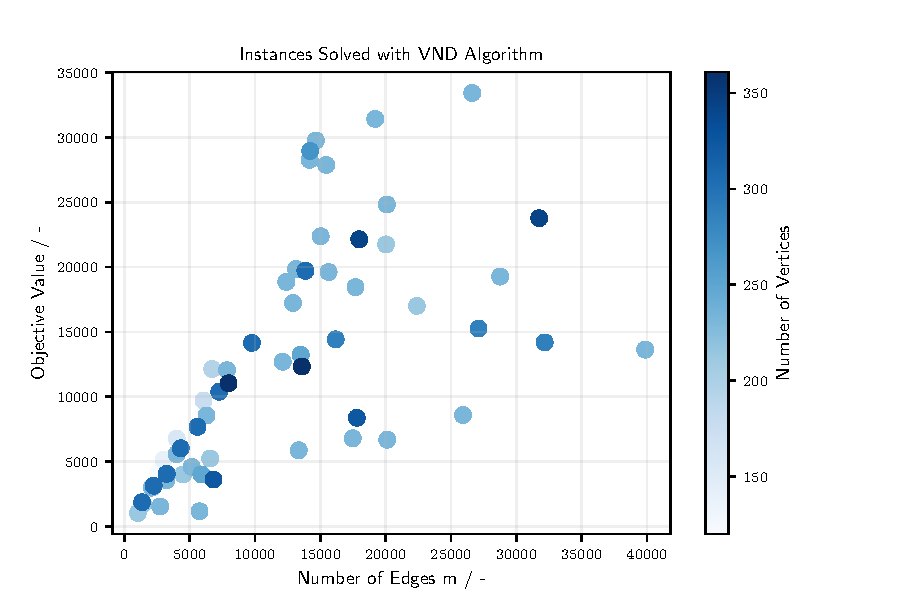
\includegraphics[width=0.7\linewidth, trim= {0 0cm 0 0cm}, clip]{figures/vnd_edges_vs_objVal.pdf}
    \caption{\label{fig:types}Linear increase in objective value with edge number, probably problem dependent}
\end{figure}

\begin{figure}[h]
    \centering
    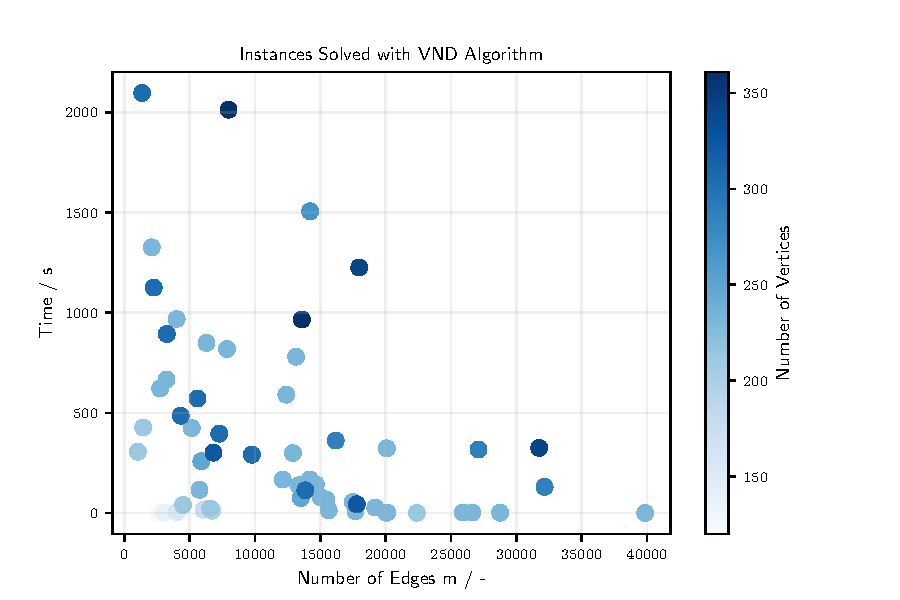
\includegraphics[width=0.7\linewidth, trim= {0 0cm 0 0cm}, clip]{figures/vnd_edges_vs_time.pdf}
    \caption{\label{fig:types}Interesting Time front, the algorithm seems to find a result faster than on smaller instances.}
\end{figure}


\section{SNS}
We ran the sequential neighbourhood search and the VND on half of the instances. You can find the results in \texttt{full\_run\_vnd.csv} and \texttt{full\_run\_sns.csv}. To our surprise is that we found that in most cases vnd is faster, in most cases not by much but still. We also found that the values are in some cases slightly different, the objective values differ by at most 60 but still.

\section{GRASP}

You can find our implementation of the GRASP algorithm in the function \texttt{grasp!}. You can find the results in \texttt{grasp.csv} and in section \ref{sec:comp_of_algos}.\\
On some instances we got better results than with vnd, but not much, and also not in many instances, so the computational effort is in our implementation not worth the improvement in the solutions. With another random construction heuristic, the improvement could be better.\\


\section{GVNS}
You can find our implementation of the GVNS algorithm in the function \texttt{gvns!}
As our shaking moves we chose to disconnect a number of random nodes totally. We found in manual testing, that for graphs of $n=300$, disconnecting $100$ and $150$ are good values, so we did our experiments with this. You can find the results in \texttt{gvns.csv} and in section \ref{sec:comp_of_algos}.\\
On some instances we got better results than with vnd, but not much, and also not in many instances, so the computational effort is in our implementation not worth the improvement in the solutions. With different shaking moves, the improvement could be better.\\

\pagebreak

\section{Manual Parameter tuning}

The relevant parameters are:
\begin{itemize}
    \item best or first improvement: Here, due to time only first improvement is relevant. We used best improvement only on the competition instances.
    \item Number of disconnected nodes in the shaking moves. We found 100 nodes in the first shaking neighbourhood and 150 nodes in the second shaknig neighbourhood to work well (at least not worse than others).
    \item Initial cluster size: Our construction heuristic has a parameter that limits the size that clusters have after construction we discussed this in section \ref{sec:basic_ideas}. Unsurprisingly, the computation time is smaller when the initial cluster size is maximal, because then the number of clusters is $n/s$ which decreases the size of our neighbourhoods as discussed in section \ref{sec:neigh}. The results seem to not be very effected by this value.
\end{itemize}
\section{Delta Evaluation}

We implemented delta evaluation, but we only did so for one case to have a working example with an estimate of the performance gain and a proof of correctness.\\
Since the structure of our functions did not really fit delta evaluation, we created new, adapted functions. The basic idea behind our delta evaluation is that for every changed bit in $A$ we calculated the added cost similar to the following pseudocode:\\
\begin{verbatim}
    changed = (G.A[i, j] == 1)
    G.A[i, j] = 0
    cost_reduced = (G.A0[i, j] == 0)
    added_cost += changed * (-cost_reduced * 2 + 1) * G.W[i,j]
\end{verbatim}
We adapted the move operators \texttt{fuse\_first!} and \texttt{swap\_first!}, you can find the adapted versions in \texttt{move\_ops\_delta.jl}. We made a new version of the VND which you can find in \texttt{metaheuristics.jl}, it is called \texttt{vnd\_delta!}.\\
We only did a quick check on the performance and correctness of our implementation of delta evaluation in \texttt{delta\_eval.jl}. If you run it you will see, that the improvement that delta evaluation made was (if at all existend) smaller than statistical fluctuations of the runtime. On our machine it takes 50 seconds to run, if you dont want to run it, the output of our machine is: (for one run, the time, of course, fluctuates statistically)
\begin{verbatim}
    ======
    Demo of Delta Evaluation
    ======
    running vnd and vnd_delta for file ../data/datasets/inst_competition/heur051_n_300_m_20122.txt
    
    Profiler of VND with fastest configuration with delta evaluation
    calculated obj value of delta evaluation is: 6930
    Actual obj value is: 6930
    Total time for VND is 3.578387975692749
    ====
    
    
    Profiler of VND with fastest configuration without delta evaluation
    Actual obj value is: 6930
    Total time for VND is 3.64827299118042
    ====
\end{verbatim}
We know that this is not good practice in terms of experimentation but we think it is sufficient to show that delta evaluation is correct and for this problem not very useful. We also ran this for other files, the results were comparable.\\






\section{Comparison of the algorithms}
\label{sec:comp_of_algos}

\begin{figure}[h]
    \centering
    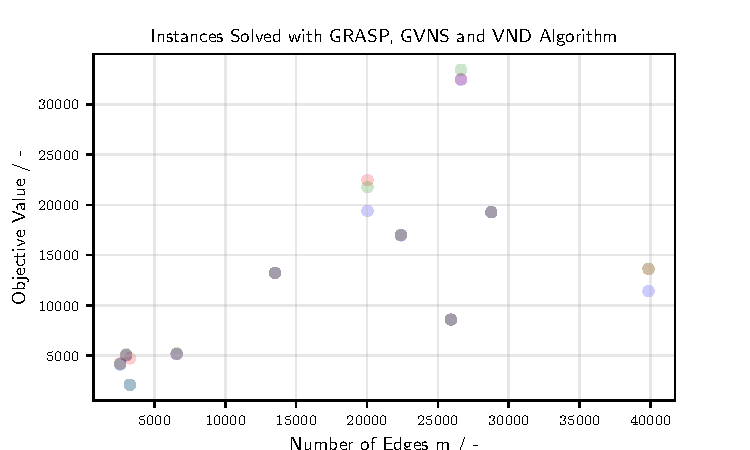
\includegraphics[width=\linewidth, trim= {0 0cm 0 0cm}, clip]{figures/vnd_grasp_gvns_edges_vs_obj.pdf}
    \caption{\label{fig:types}VND, GRASP and GVNS partial results}
\end{figure}

We also uploaded our results to the competition in tuwel.
The comparison of the algorithms is only made with the achieved objective values. There are instances where the 
GVNS actually outperforms the GRASP and VND algorithms, which is what one would expect. Due to time constraints
 we were not able to produce more conclusive results to show. Interstingly, in some instances (darker dots in the 
 figure above) some instances produced almost identical outcomes with respect to the objective value. We assume, 
 that this is an effect of our move and swap operators that we implemented.

